%!TEX root = ../thesis.tex
%*******************************************************************************
%****************************** Third Chapter **********************************
%*******************************************************************************

\chapter{Results}

% **************************** Define Graphics Path **************************
\ifpdf
    \graphicspath{{Chapter3/Figs/Raster/}{Chapter3/Figs/PDF/}{Chapter3/Figs/}}
\else
    \graphicspath{{Chapter3/Figs/Vector/}{Chapter3/Figs/}}
\fi

% Oscillations 
\section{Regulation of the CLV3 domain induces periodicity when perturbed}
When tracking the number of CLV3 nuclei identified by Costanza, the results
observable in \cref{fig:clv3_trajs} shows the number of observed CLV3 nuclei
increasing for plants 2, 4, 13, and 15, corresponding to a visually observable
enlargement of the CLV3 domain in \FIG (timelapse of example plant over 4
timepoints?). Similarly, fluctuations in this number can be seen not to 
correlate with the mean expression as described in
\cref{tab:corr_nNucl_meanExpr}. % and therefore ought to be structural

\begin{figure}[H]
  \centering
  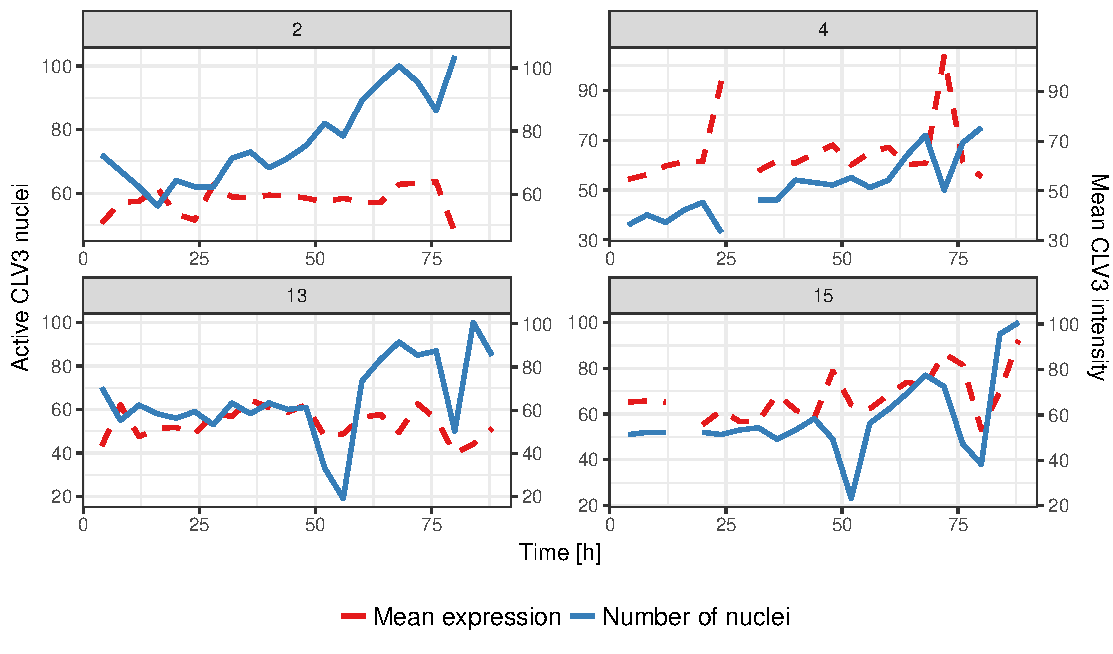
\includegraphics[width=.8\textwidth]{nNucl_trajectories.pdf}
  \caption{Add caption}
  \label{fig:clv3_trajs}
\end{figure}

\begin{table}
  \centering
  \caption{TODO}
  \label{tab:corr_nNucl_meanExpr}
  \begin{tabular}{ll}  \toprule
    Plant & p-value \\ \midrule
    2     & 0.48    \\
    4     & 0.84    \\
    13    & 0.91    \\
    15    & 0.11    \\ \midrule
    All   & 0.50    \\ \bottomrule
  \end{tabular}
\end{table}

In order to assess the extent of the fluctuations the lines were detrended using
a second order Loess fit to each curve. When performing a continuous time
Fourier transform in order to extract amplified modes, the plants have are
biased towards the fourth mode in each respective transformation, as depicted in
\cref{fig:modes}, which corresponds to periodicity of $\sim$16~hours. 

\begin{figure}[H]
  \centering
  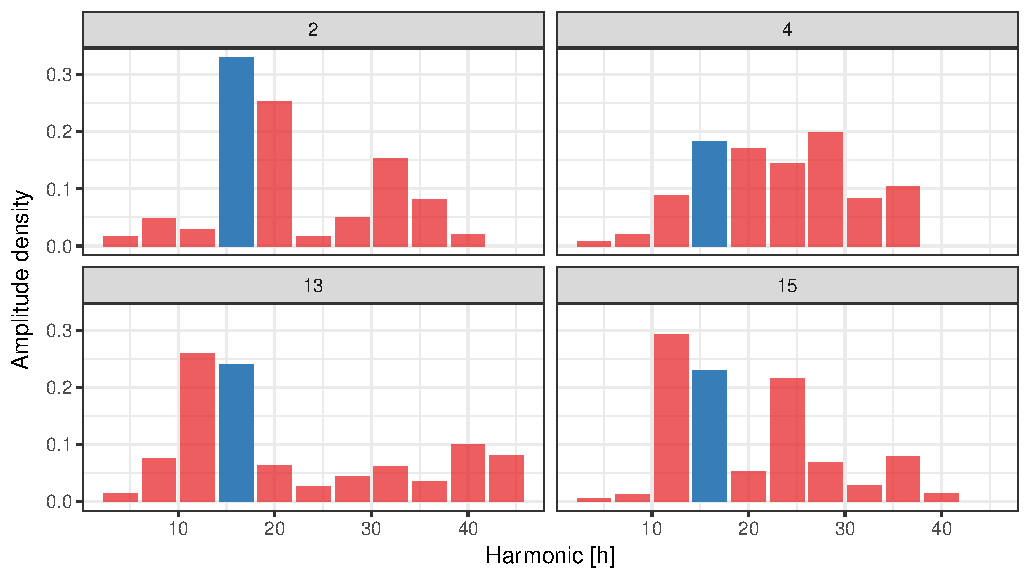
\includegraphics[width=.7\textwidth]{periodogram.pdf}
  \caption{Add caption}
  \label{fig:periodogram}
\end{figure}

\todo{map this to light / dark hour cycles?}
% and are hence not circadian

In addition to this periodicity, the number of nuclei identified correlates
positively with the number of division events observed in each timepoint for
three out of the four plants (\cref{fig:corr_nNucl_nDivs}). Plant 13, like in 
\cref{fig:clv3_trajs} is the only anomously behaving specimen.
\unsure{Should I add other correlations and just draw plots?}

\begin{figure}[H]
  \centering
  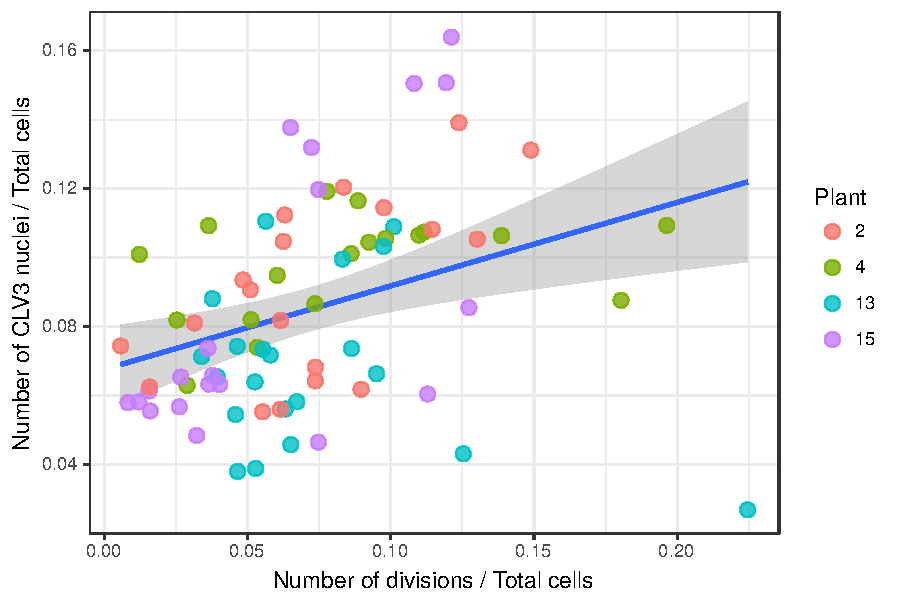
\includegraphics[width=.7\textwidth]{corr_nNucl_nDivs.pdf}
  \caption{Add caption}
  \label{fig:corr_nNucl_nDivs}
\end{figure}

\section{CLV3 noise is kept at bay at apex}

Variance in the expression of CLV3 is suppressed in the apical cells, as can be
seen in \cref{fig:expr_vs_d2t}. This appears true for all plants, although plant
in particular shows tendencies of having a few lowly expressing apical cells at
several timepoints. It should however be noted that it is possible that errors
in the tracking produces this type of data. Accounting for this possibility, all
plants have hysteresis-like shapes. Nevertheless, the distribution of expression
values at distinct distances does not appear to be bimodal, as would indicate
bistability in stem cell regulation. Instead, the data suggests an apparent CLV3
gradient, proportional to the distance to the apex more in radial terms than
in bimodal. 

Using a simple model replicating the epidermis, we are possible to replicate the
shape of the distribution assuming enzymatic CLV3 activation by a WUS gradient
(\cref{}). The enzymatic activation is in this formulation necessary in order to
attain the sigmoidal shape of the curve, where the extent of noise ultimately
depends on tha abundance of the WUS protein.
\FIG

\begin{figure}[H]
  \centering
  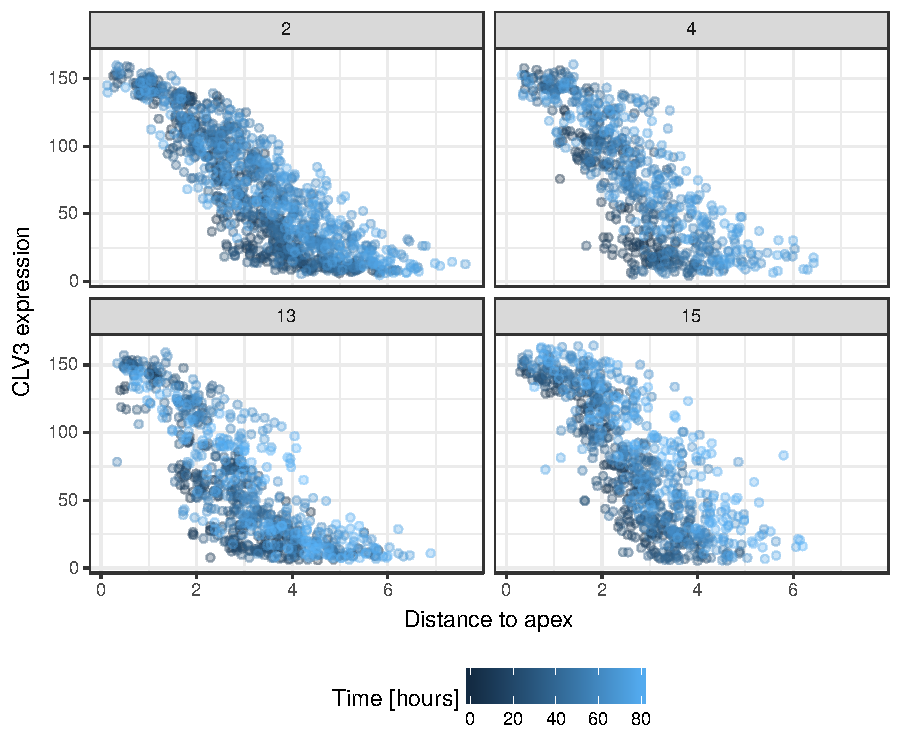
\includegraphics[width=.8\textwidth]{clv3_vs_d2t.pdf}
  \caption{Add caption}
  \label{fig:clv3d2t}
\end{figure}

A layer-wise separation of the CLV3 expression can be seen in particular between
L1 and L2, as visualised in \cref{fig:epireg}. In L1, the correlation between
CLV3 expression and nuclear volume appears sigmoidal, although consideration
should be taken to the fluorescence ceiling due to the laser. In contrast, both
L2 and L3 have linear relationships, indicating the possibility of epidermal
activation alternatively subepidermal repression altering the distributions.
Also in the distributions of CLV3 expression in relation to the distance to the
apex this effect is observable.



\begin{figure}[H]
  \centering
  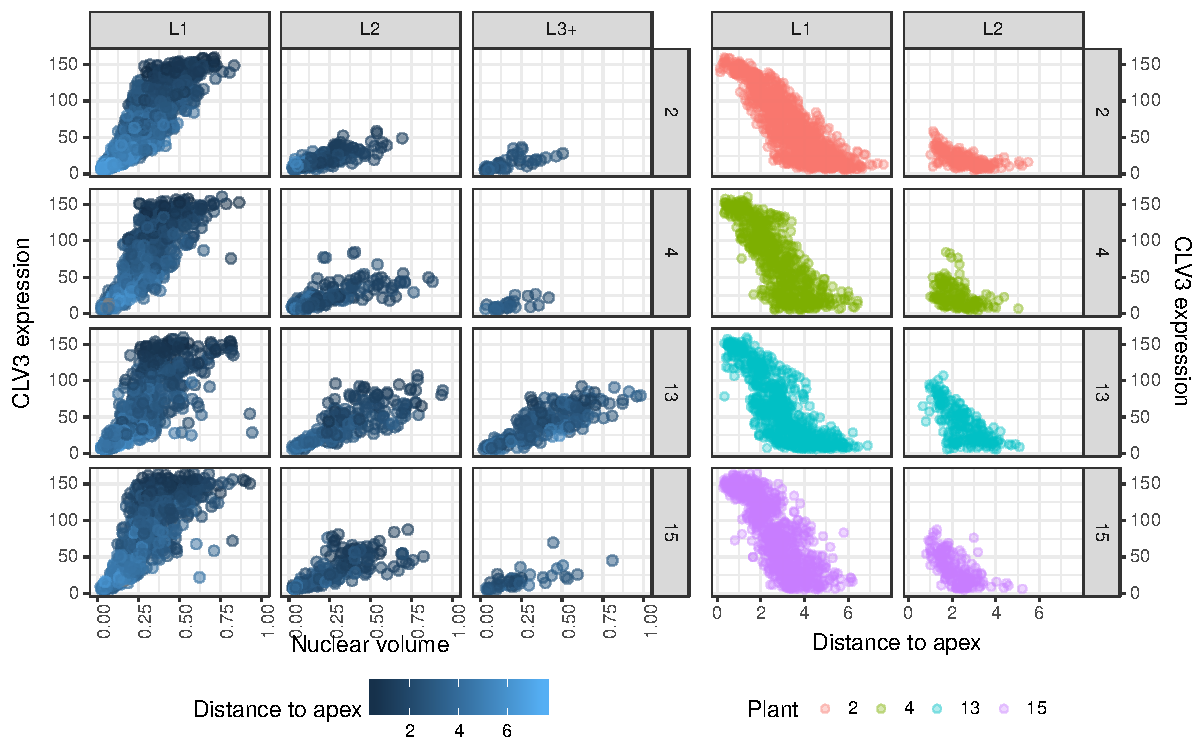
\includegraphics[width=\textwidth]{epireg.pdf}
  \caption{Add caption}
  \label{fig:epireg}
\end{figure}

%\section{Distribution shifting suggests epidermal regulation}
%\subsection{CLV3 is induced in the epidermis}




 % This holds regardless of what distribution looks like

 \section{Functional clustering implies dsRED technical artefacts}

 \begin{figure}[H]
   \centering
   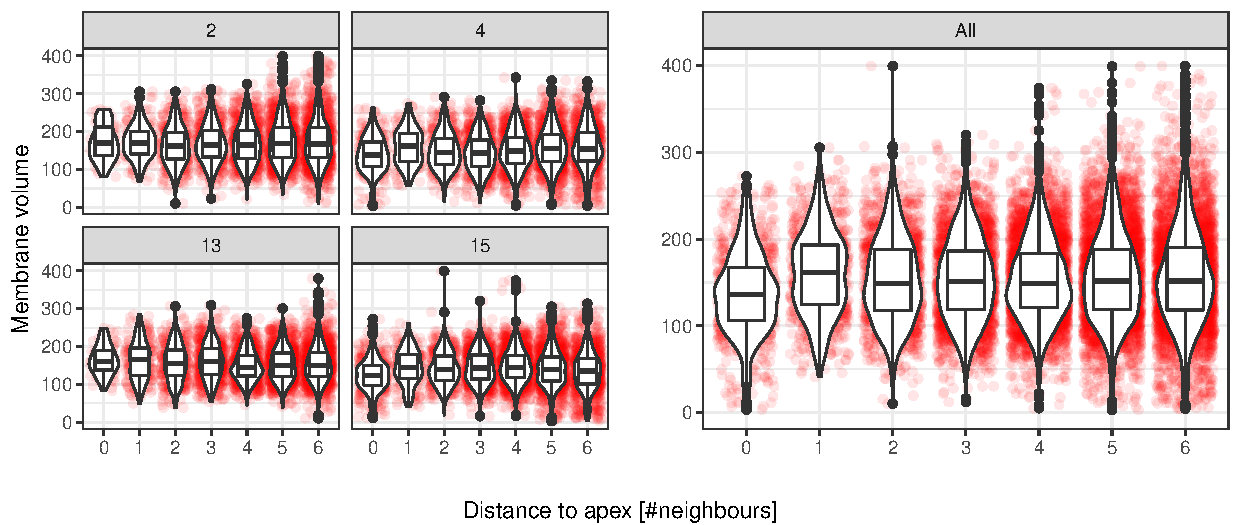
\includegraphics[width=\textwidth]{mvol_apex.pdf}
  \caption{Add caption}
  \label{fig:mvol_apex}
\end{figure}

\begin{figure}[H]
   \centering
   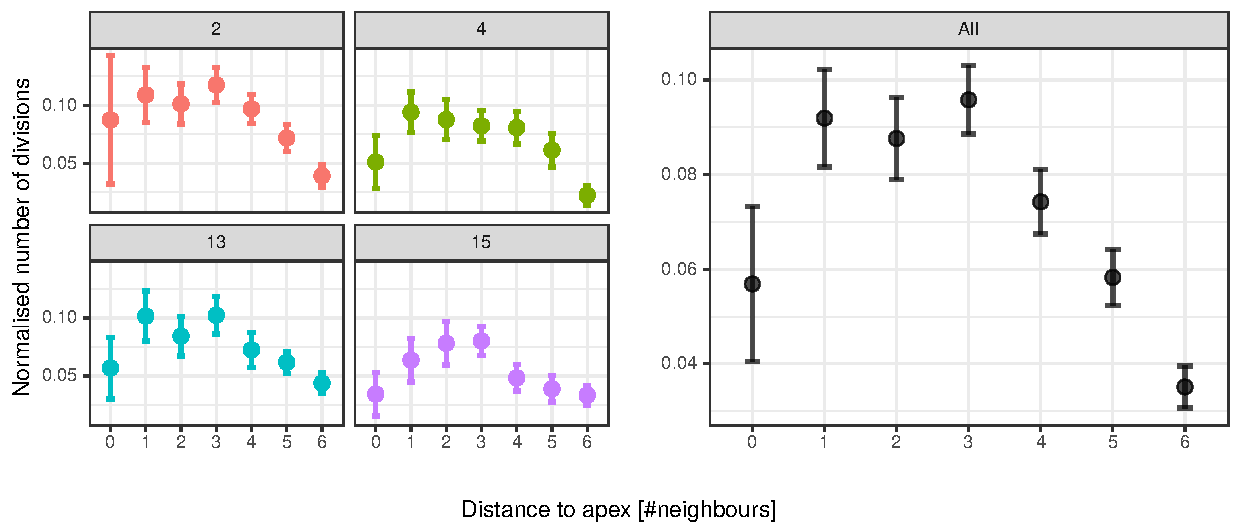
\includegraphics[width=\textwidth]{nDivs_apex.pdf}
   \caption{Add caption}
  \label{fig:mvol_apex}
\end{figure}


\begin{figure}[H]
  \centering
  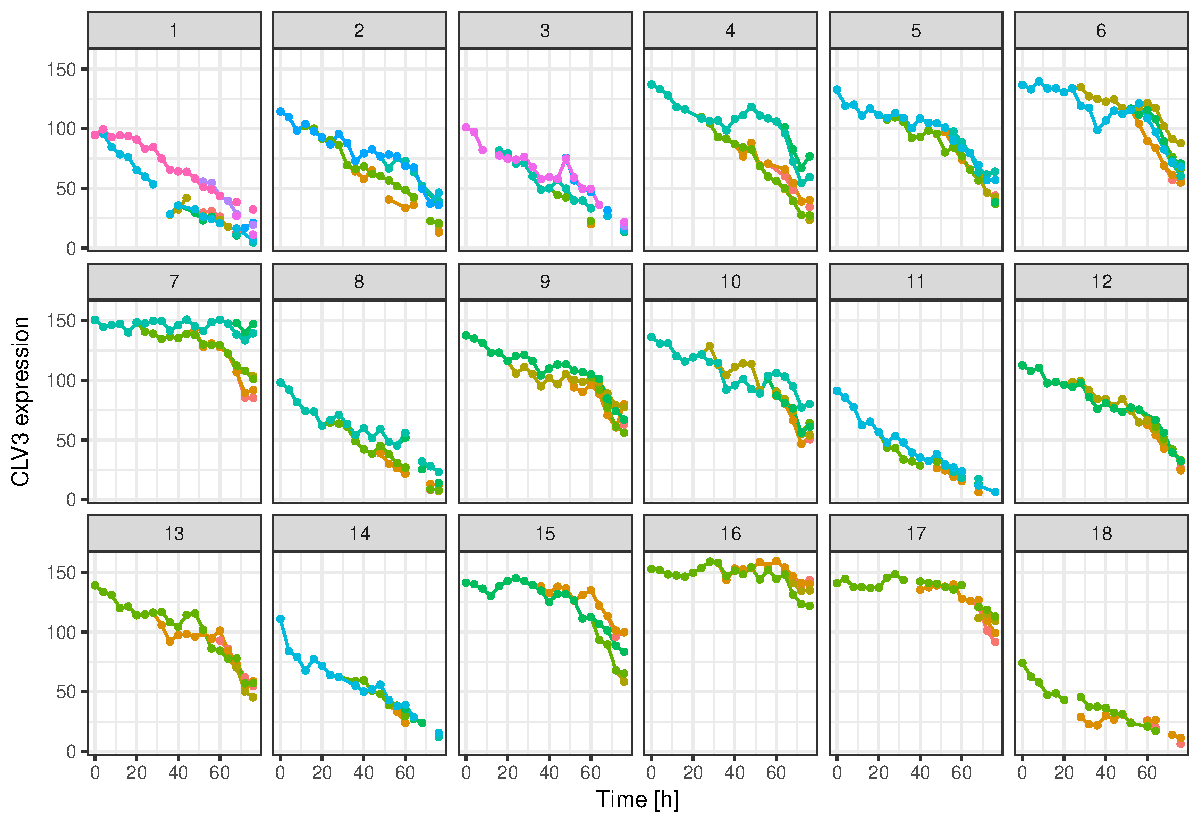
\includegraphics[width=\textwidth]{plant2_trajectories.pdf}
  \caption{Add caption}
  \label{fig:corr_nNucl_nDivs}
\end{figure}

\begin{figure}[H]
  \centering
  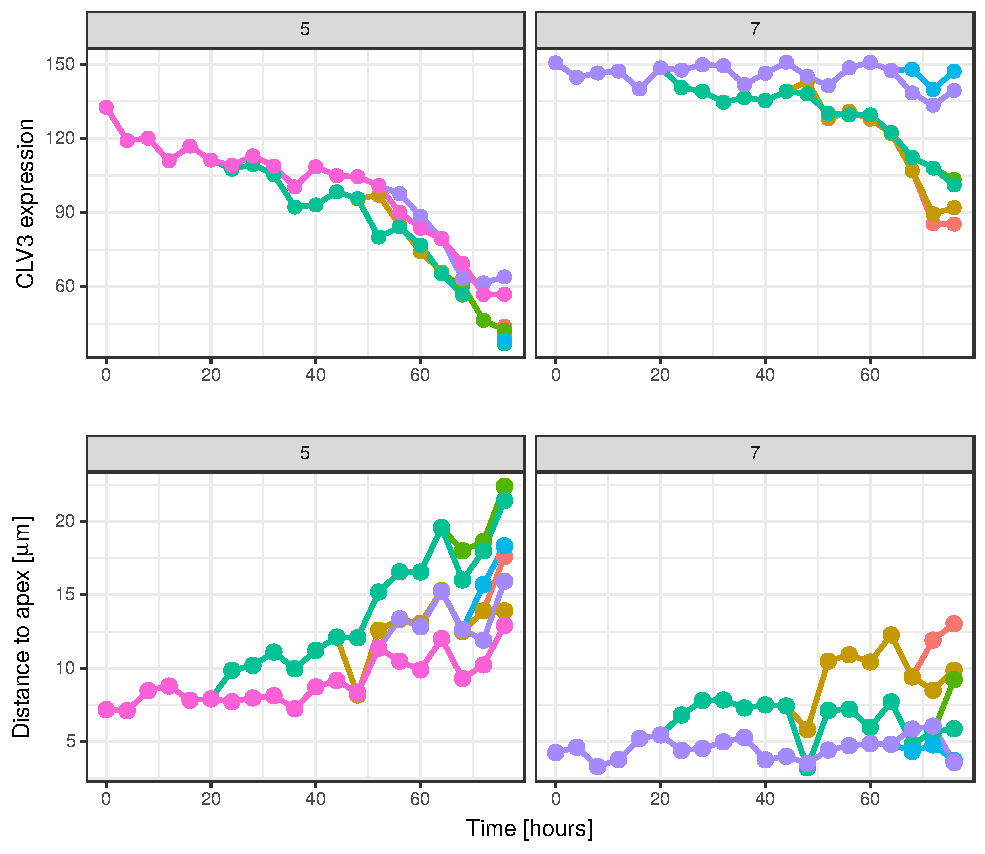
\includegraphics[width=.5\textwidth]{select_trajectories.pdf}
  \caption{Add caption. }
  \label{fig:select_trajs}
\end{figure}

\begin{figure}[H]
  \centering
  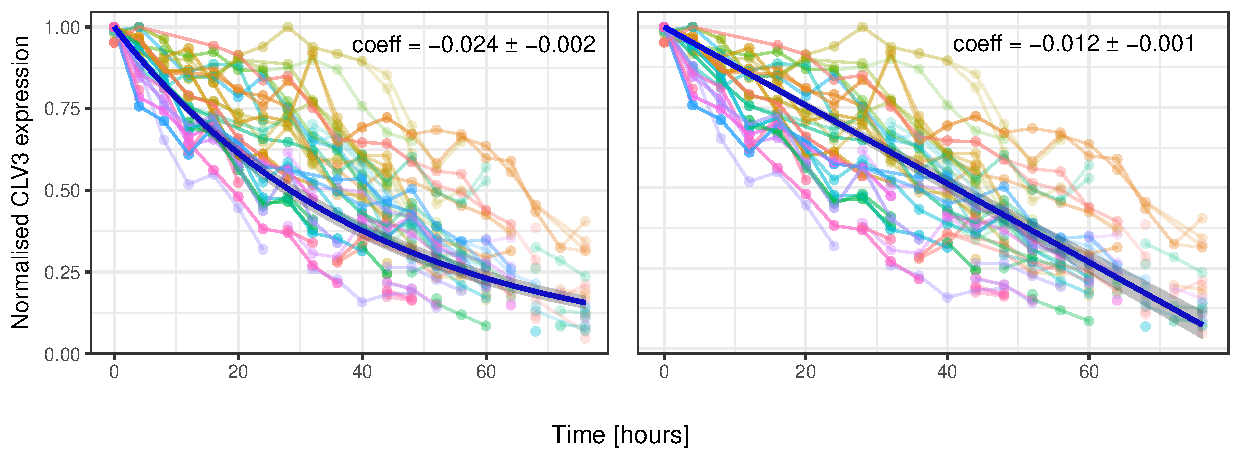
\includegraphics[width=\textwidth]{dsred_plant2.pdf}
  \caption{Add caption}
  \label{fig:dsred_decay}
\end{figure}

TODO: Justification for decay. Assume movement out of CZ proportional to
division rate $k_{div}$, such that $\dot{R} \propto k_{div}$. We thus have
$R = kt$. Assume linear degradation of CLV3 such that $\dot{C} = -k_{deg} =
\frac{\dd C}{\dd t} = \frac{\dd C}{\dd R} \frac{\dd R}{\dd t}$. We therefore have
$\frac{\dd C}{\dd R} = \frac{\dd C}{\dd t} = -\frac{k_{deg}}{k_{div}}$. Justify
decay rate observed in trajectories or smth like that?


\section{Deep-tissue cells divide at a slower rate}
Still unknown.
